\chapter{Implementacja}
\label{cha:implementacja}

Działanie programu można podzielić na dwa główne etapy. Pierwszym jest dostarczenie danych zgodnych z formatem apliakacji, drugim jest reprezentacja danych.

\section{Struktura}
\label{sec:structure}

Struktura klas w aplikacji została stworzona w oparciu o wzorzec projektowy MVC(en. Model–view–controller). Zakłada on podział na 3 główne warstwy, są nimi:

\begin{itemize}
\item
Controller - jego zadaniem jest przyjmowanie danych wejściowych i na ich podstawie odpowiednia reakcja, która może być aktualizają modelu lub warstwy prezentacyjenj.  W aplikacji funkcję tą spełniają servisy i kontrolery.
\item
View - warstwa prezentacyjna, zapewnia wizualiną prezentację infrmacji. Rolę tą w omwianym projekcie spełnia HTML i CSS.
\item
Model - przechowuje dane, stanowi bazę danych. Jego rola została przeniesiona na natywne rozwiązanie jakim jest Storage.
\end{itemize}
 
Założenia nie zostały spełnione wszystkie założenia jednak stworzono podstawy do rozwoju i prostej adaptacji rozwiązania do potrzeb konkretnego klienta.



Zastosowano również paradygmat odwrócenia sterowania(en. Inversion of control,IoC) polegający na przeniesieniu poza obiekt metod służących do kontroli poszczególnych obiektów. Główną zaletą tego podejścia jest uproszczona kongiguracja i adaptacja programu do specyficznych potrzeb. Przykładem jego zastosowania jest metoda korzystania z filtrów w aplikacji, które mogą być tworzone przez użytkownika. Ich potencjalnie duża ilość wczytywana jednocześnie podczas startu generowałaby zbędne obciążenie, obecnie są one pomijane podczas inicjacji i wczytywane pojedyńczo jedynie wtedy gdy ich obecność jest niezbędna.


Struktura klas obecnych w aplikacji została zaperzentowana na rysunku \ref{fig:classDiagram2}.

\begin{center}
\begin{figure}[H]
\centering
     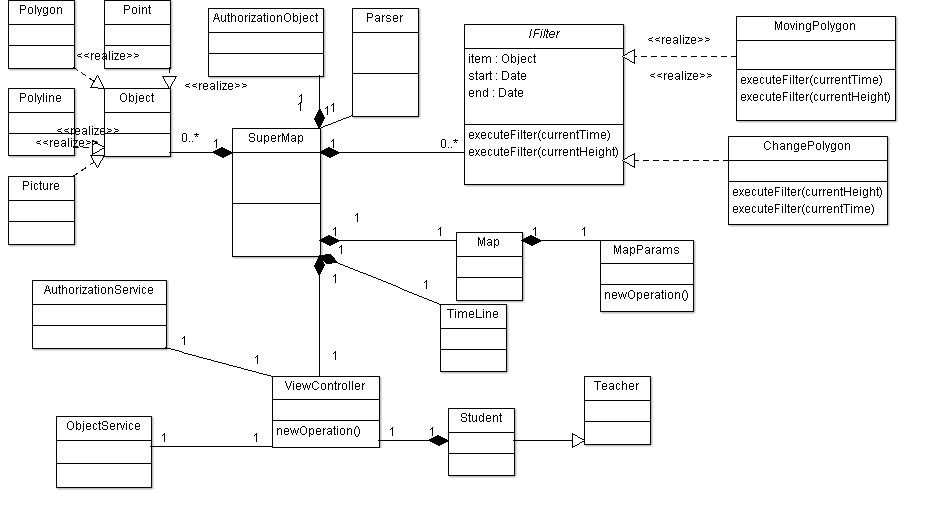
\includegraphics[angle=270,origin=c,width=130mm]{ge/smieci/ClassDiagram.png}
      \caption{Diagram klas.}
       \label{fig:classDiagram2}
\end{figure}
\end{center}

\section{Minimalna konfiguracja}
\label{sec:minimum}

Do rozpoczęcia korzystania z gotowej aplikacji należy zapewnić obecność konfiguracji niezbędnej do jej konfiguracji na docelowej stronie. Przykład minimalnej strony która spełnia wymagane został pokazany w listinu \ref{lst:minconf}.

Każdy dokument stworzony w HTML sklada się z 3 części:


-lini zawierającej informację o używanej wersji HTML, w poniższym przykładzie dotyczy ona HTML5

-deklarację sekcji header, zawiera odwołania do zewnętrzych plików i delkaracje funcji, styli

-część właściwa strony która zawiera infromacje właściwe, widoczne dla użytkownika storny.

Linie 5-7 mają za zadanie wczytanie zewnętrzych plików zawierające delkaracje metod w JS. 8 wczytuje plik zawierający główną klasę frameworku, poniżej znajduje się wczytanie niezbędnych styli CSS dla działąnia osi czasu. 13-23 jest to opis metody która inicjuje działanie mapy, jest ona wykonywana po załadowaniu statycznych fragmentów strony.

\lstset{language=JavaScript}
\begin{lstlisting}[label={lst:minconf},caption={Minimalna konfiguracja.}]

<!DOCTYPE html>
<html>
  <head>
    <script type="text/javascript" src="https://maps.googleapis.com/maps/api/js?sensor=false&key={KEY_ID}">
    <script type="text/javascript" src="./js/specialMap/lib/jquery-1.6.2.min.js"></script>
    <script type="text/javascript" src="./js/specialMap/lib/mxn/mxn.js?(googlev3)"></script>
    <script type="text/javascript" src="./js/specialMap/lib/timeline-1.2.js"></script>
    <script type="text/javascript" src="./js/specialMap/src/timemap.js"></script>
    <script type="text/javascript" src="./js/specialMap/src/utils.js"></script>

    <link type="text/css" rel="stylesheet" href="./css/examples.css"/>

    <script>
    var sm;
    $(function() {
        tm = SpecialMap.init({
            mapDivId: "mapId",
            timeDivId: "timeId",
            dataType: "sessionStorage",
            bandIntervals: [
	            Timeline.DateTime.YEAR
	        ],
        });
    });
  </head>
  <body>
        <div id="specialMap">
            <div id="timeId"></div>
            <div id="mapId"></div>
        </div>
  </body>
</html>
\end{lstlisting}/


\section{Interfers do map}
\label{sec:mxn}

W procesie badań literaturowych podjęto decyzję aby jako głównego źródła map wykorzystać Google Maps \ref{subsec:Rodzaje map}. Niestety omawiane rozwiązania posiadają różne, często niekompatybilne interfejsy do ich obsługi. Implementacja tworzonego frameworku pod wybrany typ map uniemożliwiłoby wykorzystanie innych rodzajów. Aby zaoferować możliwość wyboru zdecydowano się na wykorzystanie Mapstraction, biblioteki któej zadaniem jest płynne przechodzenie pomiędzy różnymi dostarczycielami i ich interfejsami.

Listening \ref{lst:mapstraction} pokazuję przykład wykorzystania biblioteki. Stworzenie instancji Mapstraction polega na wywołaniu konstruktora z podaniem id elementu który znajduje się na stronie i będzie używany jako nasza mapa a także typ mapy. Rezultatem jest obiekt kóry posiada wspólny interjeft dla różnych dostarzcycieli danych.

\lstset{language=JavaScript}
\begin{lstlisting}[label={lst:mapstraction},caption={Wykorzystanie Mapstraction.}]

var map = new Mapstraction(mapId, 'google');

var point = new mxn.LatLonPoint(0,0);
var marker = new mxn.Marker(point);
map.addMarker(marker);

\end{lstlisting}/



\section{Odczyt danych}
\label{sec:idata}

Tak jak zostało omówione w sekcji \ref{sec:dataformat} do przechowywania danych wybrany został format KML, jego duża popularność sprawia że stworzona aplikacja posiada dużą bazę danych z których może korzystać.

W celu odczytu i konwersji danych z pliku zapisu ich w pamięci sesyjnech przęglądarki omówionej w rozdziale \ref{subsec:storage5} stworzona została klasa KmlParser. Posiada ona jednoargumentowy konstruktor przyjmujący ciąg znakowy.

Ze względów bezpieczeństwa JavaScript nie zezwala na bezpośredni dostęp do plików lokalnych uzytkownika. Jest to pozytywne zachowanie zapewniające że żaden kod nie jest w stanie bezwiednie zmieniać zawartość dysku.

Sytuacja taka wymusza korzystanie z event-ów które będą aktywowane w momecie kiedy plik zostanie wybrany. W momencie zakończenia procesu odczytu zawartość pliku przekazywana jest do parsera który zapisuje dane w pamięci przeglądarki.

\lstset{language=JavaScript}
\begin{lstlisting}[label={lst:utils},caption={Minimalna konfiguracja.}]

var exml;
function readFile(file,start,stop){
	var reader = new FileReader();
    reader.onloadend = function(evt) {
      if (evt.target.readyState == FileReader.DONE) {
		exml = new KmlParser( evt.target.result);	
		exml.parse()
      }
    };
	
	var blob = file.slice(start, stop);
    reader.readAsBinaryString(blob);
}


\end{lstlisting}/


\lstset{language=JavaScript}
\begin{lstlisting}[label={lst:minconf},caption={Minimalna konfiguracja.}]

KmlParser.value = function(e) {
	a = GXml.value(e);
	a = a.replace(/^\s*/, "");
	a = a.replace(/\s*$/, "");
	return a;
}

KmlParser.prototype.createMarker = function(point,begin, end, name, desc, style, iconUrl) {
	var icon = {};
	var markeroptions = this.opts.markeroptions || {};
	var icontype = this.opts.icontype || "style";
	if (icontype == "style") {
		if (!!this.styles[style]) {
			icon = this.styles[style];
		}
	}
	if (!markeroptions.icon) {
		markeroptions.icon = icon;
	}
	var m = new google.maps.Marker(point, markeroptions);

	if (this.opts.elabelclass) {
		var l = new ELabel(point, name, this.opts.elabelclass,
				this.opts.elabeloffset, this.elabelopacity, true);
	}
	this.gmarkers.push(m);
	item = {};
	item.start = begin;
	item.end = begin;
	item.title = name;
	item.desc = desc;
	item.iconUrl = iconUrl;
	p = {};
	p.lat = point.lat();
	p.lon = point.lng();
	item.point = p
	return item;
}

KmlParser.prototype.createPolyline = function(points, color, width, opacity,
		name, desc) {
	var polylineoptions = this.opts.polylineoptions || {};
	var p = new GPolyline(points, color, width, opacity, polylineoptions);
	this.gpolylines.push(p);

KmlParser.prototype.createPolygon = function(points, id, pId, begin, end, color,
		width, opacity, fillcolor, fillopacity, name, desc) {

	pointsArray = []
	item = {};
	for ( var i = 0; i < points.length; i++) {
		point = points[i];
		p = {};
		p.lat = point.lat();
		p.lon = point.lng();
		if (p.lon == null || p.lat == null || isNaN(p.lat) || isNaN(p.lon)) {
			console.log("Null points");
		} else {
			pointsArray.push(p)
		}
	}
	item.start = begin;
	item.end = end;
	item.polygon = pointsArray;
	item.title = name;
	item.mId = id;
	item.pId = pId;
	item.color = color;
	item.width = width;
	item.opacity = opacity;
	item.fillcolor = fillcolor;
	item.name = name;
	item.desc = desc;

	return item;
}

KmlParser.prototype.processing = function(doc) {
	var that = this;
	var xmlDoc = GXml.parse(doc)
	
	var styles = xmlDoc.documentElement.getElementsByTagName("Style");
	for ( var i = 0; i < styles.length; i++) {
			//wczytanie styli
	}

	var placemarks = xmlDoc.documentElement.getElementsByTagName("Placemark");
	items = [];
	itemsMarkers = [];
	for ( var i = 0; i < placemarks.length; i++) {
		var id = placemarks[i].getAttribute('id');
		var timeSpan = placemarks[i].getElementsByTagName("TimeSpan")[0];
		var begin = KmlParser.value(timeSpan.getElementsByTagName('begin')[0])
		var end = KmlParser.value(timeSpan.getElementsByTagName('end')[0])
		var name = KmlParser.value(placemarks[i].getElementsByTagName("name")[0]);
		var desc = KmlParser.value(placemarks[i]
				.getElementsByTagName("description")[0]);
		if (desc == "") {
			var desc = KmlParser
					.value(placemarks[i].getElementsByTagName("text")[0]);
			desc = desc.replace(/\$\[name\]/, name);
			desc = desc.replace(/\$\[geDirections\]/, "");
		}
		if (desc.match(/^http:\/\//i)) {
			desc = '<a href="' + desc + '">' + desc + '</a>';
		}
		if (desc.match(/^https:\/\//i)) {
			desc = '<a href="' + desc + '">' + desc + '</a>';
		}
		var style = KmlParser.value(placemarks[i]
				.getElementsByTagName("styleUrl")[0]);
		var coords = GXml.value(placemarks[i]
				.getElementsByTagName("coordinates")[0]);

		var path = coords.split(" ");

		multiGeometry = getChildrenTag(placemarks[i], 'MultiGeometry')[0];
		if(multiGeometry){
			allPolygons = multiGeometry.getElementsByTagName("Polygon")
		}else{
			allPolygons = {};
		}
		
		onePoint = getChildrenTag(placemarks[i], 'Point')[0];
		if (!!that.styles[style]) {
					var width = that.styles[style].width;
					var color = that.styles[style].color;
					var opacity = that.styles[style].opacity;
					var fillopacity = that.styles[style].fillopacity;
					var fillcolor = that.styles[style].fillcolor;
					var iconUrl = that.styles[style].iconUrl;
				} else {
					var width = 5;
					var color = "#0000ff";
					var opacity = 0.45;
					var fillopacity = 0.25;
					var fillcolor = "#0055ff";
				}
		
		if(onePoint){
			coords = GXml.value(onePoint.getElementsByTagName("coordinates")[0]);
				var bits = coords.split(",");
				var point = new google.maps.LatLng(parseFloat(bits[1]),
						parseFloat(bits[0]));
				that.bounds.extend(point);
					itemsMarkers.push(that.createMarker(point ,begin,end, name, desc, style, iconUrl));
		}
		
		for ( var j = 0; j < allPolygons.length; j++) {
			polygon = allPolygons[j];
			coords = GXml.value(polygon.getElementsByTagName("coordinates")[0]);
			path = coords.split(" ");

			if (path.length > 1) {
				var points = [];
				var pId = polygon.getAttribute('id');
				for ( var p = 0; p < path.length; p++) {
					var bits = path[p].split(",");
					if (parseFloat(bits[1]) == null
							|| parseFloat(bits[0]) == null
							|| isNaN(parseFloat(bits[1]))
							|| isNaN(parseFloat(bits[0]))) {
					} else {
						var point = new google.maps.LatLng(parseFloat(bits[1]),
								parseFloat(bits[0]));
						points.push(point);
					}
				}
				this.pointsCount  = this.pointsCount + points.length;
				var linestring = placemarks[i]
						.getElementsByTagName("LineString");
				if (linestring.length) {
						that.createPolyline(points, color, width, opacity,
								name, desc);
				}

				var polygons = placemarks[i].getElementsByTagName("Polygon");
				items.push(that.createPolygon(points, id, pId, begin, end,
						color, width, opacity, fillcolor, fillopacity,
						name, desc));
			} else {
				var bits = path[0].split(",");
				var point = new google.maps.LatLng(parseFloat(bits[1]),
						parseFloat(bits[0]));
				that.bounds.extend(point);
					that.createMarker(point, name, desc, style);
			}
		}
	}
	sessionStorage.polyline = JSON.stringify(items);
	sessionStorage.marker = JSON.stringify(itemsMarkers);
}

\end{lstlisting}/

\subsection{Wydajność}
\label{subsec:wydajnosc}

W celach sprawdzenia wydajności zaimplementowanego parsera przeprowadzono testy porównawcze. W pierwszej próbie wykorzystano dwa pliki zawierające dane w formacie który pozwolił na jego analizę, pierwszy "plik1.kml" składał się z jednego obszaru i jednego stylu określającego preferencje graficzne, jego dokładana zawartość została zawarta w załączniku \ref{sec:akml}. Drugi plik "plik2.kml" zawierał informacje o granicy wszystkich stanów USA, na potrzeby badań on również zawierał informacje o jednym stylu.
Wykonano proces wczytania ich zawartości, mierząc za każdym razem czas potrzebny na zakończenie procesu. Wyniki zamieszczono w zbiorczej tabeli \ref{tab:speedTest}.

Dokładne informacje dotyczące zawartości plików zamieszczono w tabeli \ref{tab:testFile}

\begin{table}[H]
    \centering
    \begin{tabular}{|l|l|l|}
    \hline
    Nazwa pliku & Ilość punktów & Ilość poligonów \\ \hline
    plik1.kml & 13 & 1 \\ \hline
    plik2.kml & 13697 & 133 \\ \hline

    \end{tabular}
    \caption{Pliki testowe}
    \label{tab:testFile}
\end{table}


\begin{table} [H]
    \centering
    \begin{tabular}{|l|l|l|}
    \hline
    Test & 13 punktów & 12697 punktów \\\hline
    I & 3 & 343 \\\hline
    II & 13 & 449 \\\hline

    \end{tabular}
    \caption{Czas dostępu [ms]}
    \label{tab:speedTest}
\end{table}



\section{Reprezentacja danych}
\label{sec:datareprezentaction}

Posiadając już informacje należało wybrać najlepszy sposób umożliwiający ich przedstawienie. Wykorzystanie w tym celu możliwości dostarczanych przez HTML5 wydawało się bardzo zachęcające. Przykład przedstawiony na rysunku \ref{fig:canvas1} pokazuje w jak prosty sposób można zaznaczyć okrąg na gotowym obrazie. Niestety ze względu na brak kompatybilności tego rozwiązania z wybranym sposobem dostarczania informacji geograficznych sposób tworzenia kształtów został zmieniony inny.

\subsection{Rysowanie kształtów}
\label{subsec:drawpoly}

Aplikacja umożliwa tworzenie różnych kształtów i pojedyńczych elementów które można umieścić na mapie. Wykorzystywane są obiekty z pakiety google.maps, zawiera takie elementy jak:

\begin{itemize}
\item
Marker
Pozwala on na umieszczenie pojedyńczego punktu na mapie. Możliwe jest dokładne sprecyzowanie jego wyglądu dzięki czemu możliwe jest aby prezentował on określą ikonę lub symbol.
\item
Okrąg
Pierwszy kształt, tworzy idealy okrąg.
\item
Poligon
Jedna z bardziej przydatnych opcji. Dzięki niemu możemy stworzyć każdy kształt. To ten element został wykorzystany do stwrozenia granicy wyspy zaprzezentowany w załączniku \ref{sec:aresult}.
\item
Linia
Elemnt pozwalający na tworzenie lini, której wygląd możemy swobodnie określać.
\item
Prostokąt
Ostatni element tworzy prostokąty o kątach dokłanie 90 stopni. Kształt ten można próbować stworzyć przy pomocy poligonu, nie będzie on jednak tak dokładny jak przy pomocy tej opcji.

\end{itemize}

\subsection{Dodawanie filtrów}
\label{subsec:filters}

Rozwinięciem podstawowej możliwości tworzenia prostych kształtów geometrycznych jest opcja tworzenia filtrów które mogą wpływać na prezentację danych.

Przykładowym użyciem jest możliwość stworzenia animacji płynnego przejścia z jednego kształtu w inny. Proces ten jest wykonany w następujących krokach:

\begin{itemize}
\item
Przekazanie do aplikacji kształtu zawierającego informacje o stanie początkowym i końcowym.
\item
Dla każdej zmiany daty obliczenie aktualnego procentowego zakończenia procesu transformacji, gdzie pomiędzy startem a końcem okresu zmiany kształtu obecnie się znajdujemy.
\item
Oblicznie położenia nowego punktu, tak aby leżał pomiędzy dwoma w stosunku oblicoznym w poprzednim kroku.
\end{itemize}

\lstset{language=JavaScript}
\begin{lstlisting}[label={lst:minconf},caption={Minimalna konfiguracja.}]

var percent;
if (now < start) percent = 0;
else if (now > end) percent = 1;
else percent = 1 - ((end - now) / (end - start));

for (var x=0; x<pm.points.length; x++) {
    pt1 = pm.points[x];
    pt2 = ep[x];
    points.push(new mxn.LatLonPoint(
        (pt1.lat + ((parseFloat(pt2.lat) - pt1.lat) * percent)),
        (pt1.lng + ((parseFloat(pt2.lon) - pt1.lng) * percent))
    ));

\end{lstlisting}/

Istnieje możliwość tworzenia nowych filtrów dla potrzeb konkretnych map lub danych. Nie stanowi dużym problemem imlementacja takiego rozwiąznaia które w pewnym momencie wyświetliłoby krótki film wideo dostarczający dodatkowych informacji o obserwowanym wydarzeniu.

\subsubsection{Google DrawingManager}
\label{subsubsec:svg}
